%%%%%%%%%%%%%%%%%%%%%%% file template.tex %%%%%%%%%%%%%%%%%%%%%%%%%
%
% This is a template file for Web of Conferences Journal
%
% Copy it to a new file with a new name and use it as the basis
% for your article
%
%%%%%%%%%%%%%%%%%%%%%%%%%% EDP Science %%%%%%%%%%%%%%%%%%%%%%%%%%%%

\documentclass{webofc}
% option "twocolumn" for typesetting an article in two columns format (default one column)
% \documentclass[twocolumn]{webofc}

\usepackage[varg]{txfonts}   % Web of Conferences font
\usepackage{hyperref}
\usepackage{url}
%%%%%%%%%%%%%%%%%%%%%%%%%%%%%%%%%%%%%%%%%%%%%%%%%%%%%%%%%%%%%%%%%%%%%%%%%%%%%
\hypersetup{colorlinks=true,citecolor=blue,urlcolor=blue,linkcolor=blue}
%%%%%%%%%%%%%%%%%%%%%%%%%%%%%%%%%%%%%%%%%%%%%%%%%%%%%%%%%%%%%%%%%%%%%%%%%%%%%
%
% Put here some packages required or/and some personnal commands
%
%
\begin{document}
%
\title{Next-Generation Triggers for CMS at the HL-LHC: Toward Offline-Quality Real-Time Reconstruction}
%
% subtitle is optionnal
%
%%%\subtitle{Do you have a subtitle?\\ If so, write it here}

\author{
    \firstname{Bruno} \lastname{Alves}\inst{1} \fnsep\thanks{\email{bruno.alves@cern.ch}} for the CMS collaboration
}

\institute{
    CERN, 1211 Geneva 23, Switzerland
}

\abstract{The Next-Generation Trigger (NGT) program for the CMS High Level Trigger (HLT) aims at enabling full-rate recording of all the events accepted by the Level-1 Trigger at 750 kHz via a dedicated NGT Scouting stream, performing complete physics event reconstruction with no additional filtering. Reconstructed objects are stored directly in a lightweight NanoAOD format, delivering analysis-ready data at unprecedented throughput while minimizing per-event footprint. To guarantee offline-quality physics performance without storing raw detector information, major advances in HLT reconstruction have been introduced. The Patatrack pixel-tracking upgrade — extended to the first macro-pixel layers of the Outer Tracker — yields higher efficiency across the detector, sharply reduced fake rates, and substantial timing gains by eliminating a full Kalman Filter-based iteration in scouting-like menus. In addition, the streamlined HLT muon chain, based on single L1-seeded Inside-Out tracking with targeted recovery, achieves improved purity and lower computational cost in high-pileup conditions. Together, these developments enable real-time production of offline-quality objects at extreme trigger rates, opening new discovery potential for signatures currently limited by bandwidth.
}
%
\maketitle
%
\section{Introduction}
\label{intro}
Your text comes here. Separate text sections with
\section{Section title}
\label{sec-1}
For bibliography use \cite{RefJ}, \cite{RefB}
\subsection{Subsection title}
\label{sec-2}
Don't forget to give each section, subsection, subsubsection, and
paragraph a unique label (see Sect.~\ref{sec-1}).

For one-column wide figures use syntax of figure~\ref{fig-1}
\begin{figure}[h]
% Use the relevant command for your figure-insertion program
% to insert the figure file.
\centering
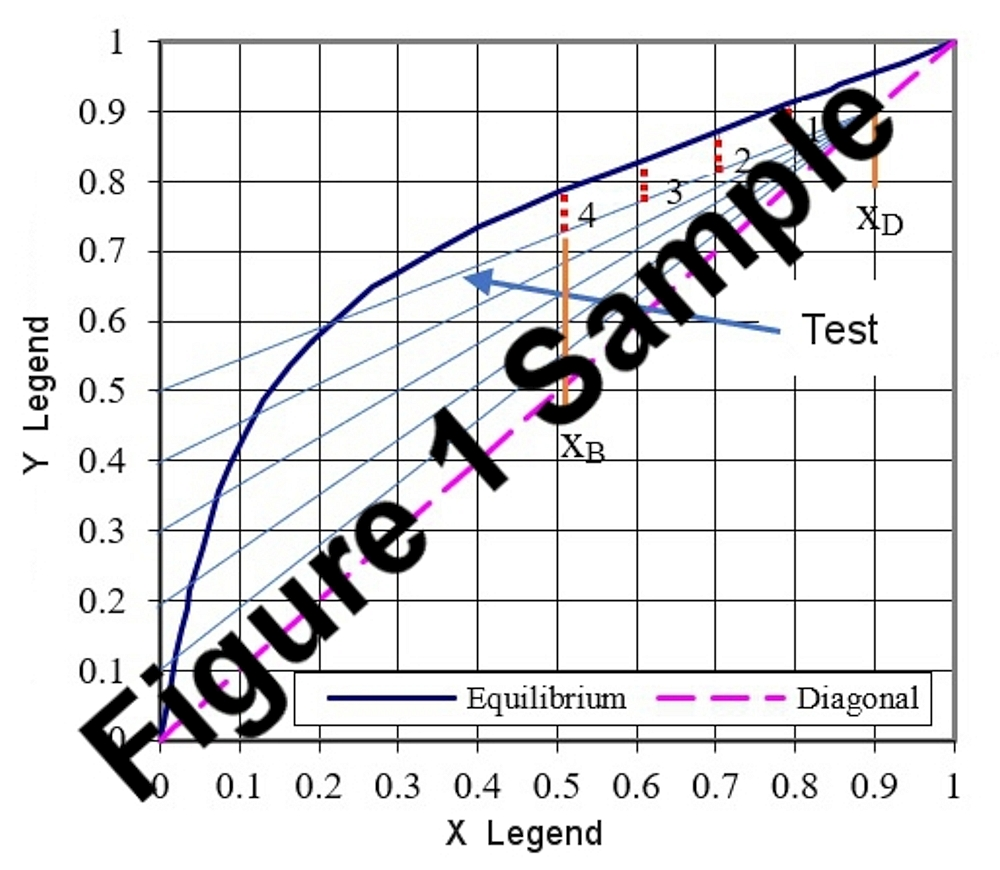
\includegraphics[width=5cm,clip]{fig-1-sample}
\caption{Please write your figure caption here}
\label{fig-1}       % Give a unique label
\end{figure}

For two-column wide figures use syntax of figure~\ref{fig-2}
\begin{figure*}
\centering
% Use the relevant command for your figure-insertion program
% to insert the figure file. See example above.
% If not, use
\vspace*{1cm}       % Give the correct figure height in cm
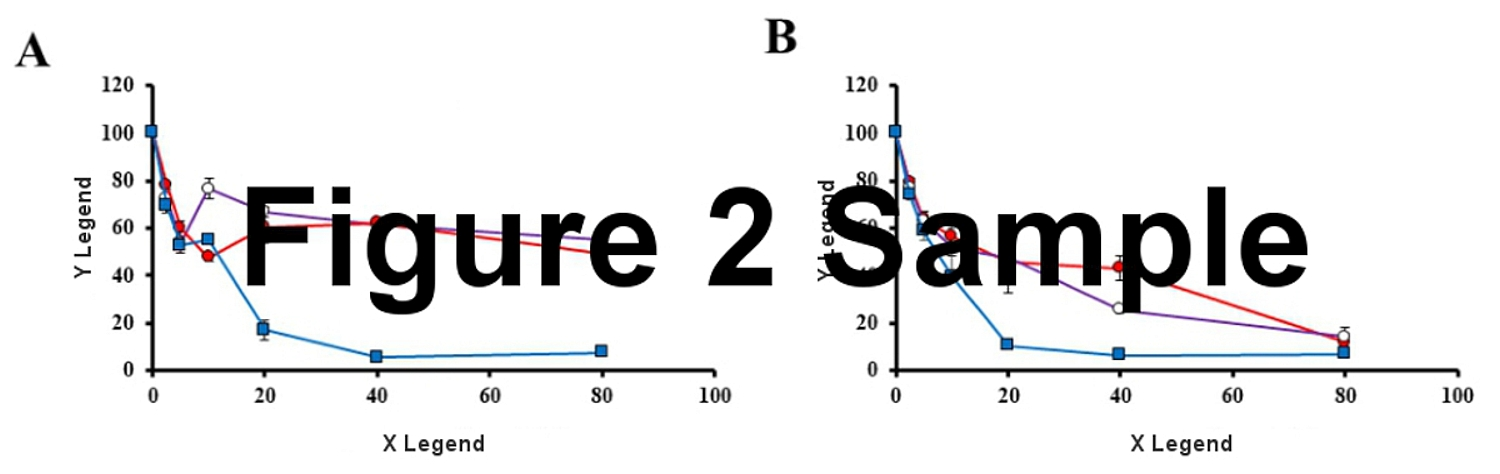
\includegraphics[width=8cm,clip]{fig-2-sample}
\caption{Please write your figure caption here}
\label{fig-2}       % Give a unique label
\end{figure*}

For figure with sidecaption legend use syntax of figure~\ref{fig-3}
\begin{figure}
% Use the relevant command for your figure-insertion program
% to insert the figure file.
\centering
\sidecaption
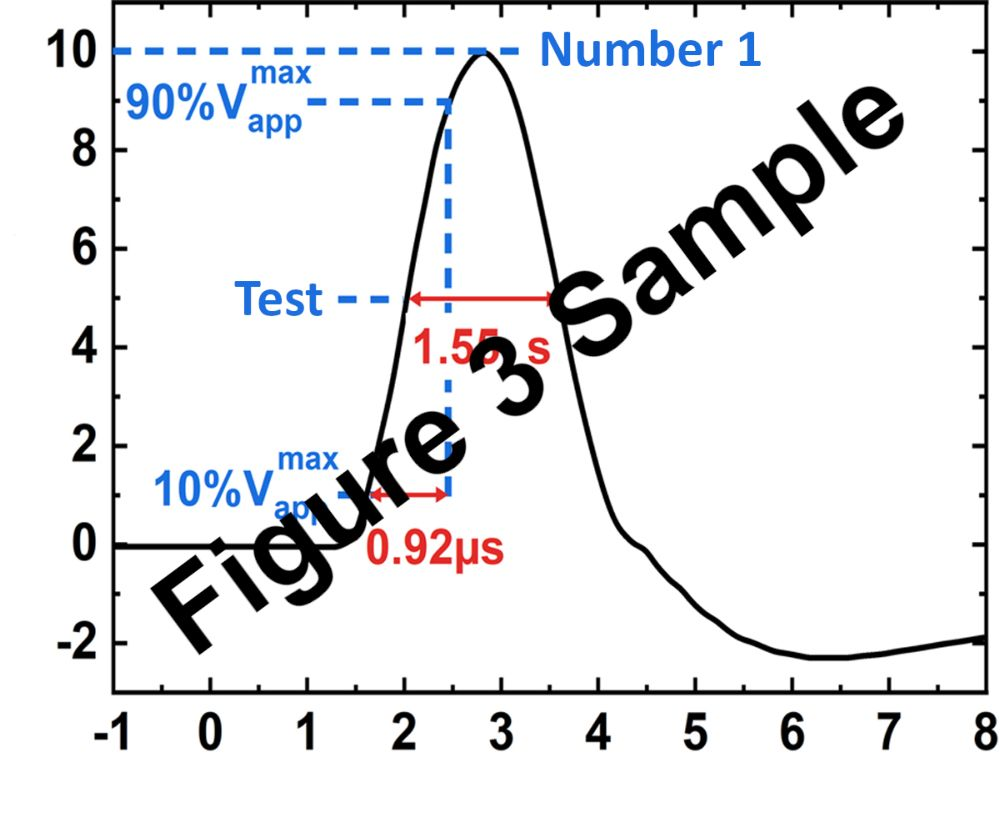
\includegraphics[width=5cm,clip]{fig-3-sample}
\caption{Please write your figure caption here}
\label{fig-3}       % Give a unique label
\end{figure}

For tables use syntax in table~\ref{tab-1}.
\begin{table}
\centering
\caption{Please write your table caption here}
\label{tab-1}       % Give a unique label
% For LaTeX tables you can use
\begin{tabular}{lll}
\hline
first & second & third  \\\hline
number & number & number \\
number & number & number \\
number & number & number \\\hline
\end{tabular}
% Or use
\vspace*{5cm}  % with the correct table height
\end{table}
%
% BibTeX or Biber users please use (the style is already called in the class, ensure that the "woc.bst" style is in your local directory)
% \bibliography{your_bib_file} % Replace "your_bib_file" with the actual name of your .bib file
%
% Non-BibTeX users please use
%
\begin{thebibliography}{}
%
% and use \bibitem to create references.
%
\bibitem{RefJ}
% Format for Journal Reference
Journal Author, Article title. Journal \textbf{Volume}, page numbers (year). \url{https://doi.org/Article-DOI-number}
% Format for books
\bibitem{RefB}
Book Author, \textit{Book title} (Publisher, place, year) page numbers
% etc
\end{thebibliography}

\end{document}

% end of file template.tex

<div id='footer'><table width='100%'><tr><td class='right'><a href='http://fusioninventory.org/'><span class='copyright'>FusionInventory 9.1+1.0 | copyleft <img src='/glpi/plugins/fusioninventory/pics/copyleft.png'/>  2010-2016 by FusionInventory Team</span></a></td></tr></table></div>